\chapterimage{blue18.jpeg} % Imagen de encabezado de capítulo
\chapterspaceabove{6.75cm} % Espacio en blanco desde la parte superior de la página hasta el título del capítulo en las páginas del capítulo
\chapterspacebelow{7.25cm} % Cantidad de espacio en blanco vertical desde el margen superior hasta el comienzo del texto en las páginas de los capítulos

%------------------------------------------------

\chapter{EL PRINCIPIO DE INCLUSIÓN Y EXCLUSIÓN}

El Principio de Inclusión y Exclusión es una herramienta esencial en combinatoria y teoría de conjuntos, utilizada para contar elementos en conjuntos que pueden tener intersecciones. La génesis de este principio se atribuye al matemático francés François Joseph Servois, quien, a principios del siglo XIX, formuló un enfoque sistemático para abordar problemas de conteo que involucran la intersección de conjuntos. Desde entonces, el Principio de Inclusión y Exclusión ha evolucionado y se ha convertido en un componente esencial del arsenal matemático en contextos discreto y combinatorio.

En su esencia, este principio se basa en un enfoque sistemático que aborda la inclusión y exclusión de elementos. La \textit{inclusión} implica considerar los elementos que pertenecen a al menos uno de los conjuntos dados, mientras que la \textit{exclusión} consiste en eliminar las sobrecontabilizaciones, es decir, los elementos que podrían estar presentes en más de un conjunto.

Al aplicar el Principio de Inclusión y Exclusión a la unión de conjuntos, se sigue un proceso secuencial. Inicialmente, se suma el tamaño de cada conjunto individual. Luego, se restan las intersecciones de pares de conjuntos para corregir posibles duplicaciones. Finalmente, se suman las intersecciones de conjuntos triples y continúa el proceso para conjuntos mayores, garantizando así que cada elemento sea contado exactamente una vez.

Este principio encuentra aplicaciones en diversos campos matemáticos. En combinatoria, permite abordar problemas de conteo desafiadores al considerar las distintas formas en que los elementos pueden interrelacionarse. En teoría de números, se utiliza para analizar propiedades combinatorias de números enteros. Además, en probabilidad, el principio se aplica para calcular la probabilidad de eventos que pueden ocurrir simultáneamente.

La versatilidad del Principio de Inclusión y Exclusión lo convierte en una herramienta fundamental para resolver problemas que involucran conjuntos superpuestos. Su comprensión profunda no solo facilita el manejo de situaciones complejas de conteo, sino que también proporciona una base conceptual sólida para abordar una amplia gama de problemas matemáticos. 

\section{El principio de inclusión y exclusión}

En esta sección desarrollaremos algo de notación para enunciar nuestro nuevo principio de conteo. Después demostraremos este nuevo principio por medio de inducción matemática (vea el \hyperref[ch:induccion]{Ápendice A}). Motivaremos con una serie de tres ejemplos.%los dos primeros recordarán el trabajo que hicimos con el conteo y los diagramas de Venn en la sección 3.3.

\begin{myexample}
    Sea $S$ el conjunto de 100 estudiantes inscritos en el primer año de ingeniería en el Instituto Politécnico Nacional. Entonces $|S| = 100$. Ahora sean $c_1$, $c_2$ las siguientes condiciones (o propiedades) satisfechas por algunos de los elementos de $S$:
    \begin{align*}
        c_1 &: \text{ Un estudiante del IPN entre los 100 estudiantes de ingeniería y está inscrito en Cálculo.} \\
        c_2 &: \text{ Un estudiante del IPN entre los 100 estudiantes de ingeniería y está inscrito en Economía.}
    \end{align*}
    Supongamos que 35 de estos 100 estudiantes están inscritos en Cálculo y que 30 de ellos están inscritos en Economía. Denotaremos esto por
    $$N(c_1) = 35 \quad \text{ y } \quad N(c_2) = 30.$$
    Si nueve de estos 100 estudiantes están inscritos tanto en Cálculo como en Economía, entonces escribimos $N(c_1 c_2) = 9$.

    Además, de estos 100 estudiantes, hay $100 - 35 = 65$ que no están tomando Cálculo. Denotando $|S|$ por $N$, podemos designarlo escribiendo $N(\bar{c}_1) = N - N(\bar{c}_1)$. De manera similar designamos que hay
    $$N(\bar{c}_2) = N - N(\bar{c}_2) = 100 - 30 = 70$$
    de estos estudiantes que no están tomando Economía. El número que están tomando Cálculo y que no están tomando Economía es
    $$N(c_1 \bar{c}_2) = N(c_1) - N(c_1 c_2) = 35 - 9 = 26.$$
    Asimismo, de estos 100 estudiantes, hay
    $$N(\bar{c}_1 c_2) = N(c_2) - N(c_1 c_2) = 30 - 9 = 21$$
    que están inscritos en Economía pero no en Cálculo. De particular interés son aquellos estudiantes (de entre estos 100 estudiantes de primer año) que no están tomando ni Cálculo ni Economía, es decir, no están tomando Cálculo y tampoco están tomando Economía. Su número es $N(\bar{c}_1 \bar{c}_2)$. Y como $N(\bar{c}_1) = N(\bar{c}_1 c_2) + N(\bar{c}_1 \bar{c}_2)$, se sigue que
    $$N(\bar{c}_1 \bar{c}_2) = N(\bar{c}_1) - N(\bar{c}_1 c_2) = 65 - 21 = 44.$$
    
    Las observaciones anteriores también demuestran que
    \begin{align*}
        N(\bar{c}_1 \bar{c}_2) & = N(\bar{c}_1) - N(\bar{c}_1 c_2) \\
        & = [N - N(c_1)] - [N(c_2) - N(c_1c_2)] \\
        %& = N - N(c_1) - N(c_2) + N(c_1 c_2) \\
        & = N - [N(c_1) + N(c_2)] + N(c_1 c_2) \\
        & = 100 - [35 + 30] + 9 = 44, \text{ como vimos anteriormente.}
    \end{align*}
    \begin{minipage}[l]{0.6\textwidth}
        En el diagrama de Venn de la figura \ref{IAIAOAOAIJSJBJSKSI}, vemos que si $N(c_1)$ denota el número de elementos de $S$ en el círculo de la izquierda y $N(c_2)$ denota el número en el círculo de la derecha, entonces $N(c_1 c_2)$ es el número de estos elementos de $S$ en la intersección, mientras que $N(\bar{c}_1 \bar{c}_2)$ cuenta aquellos elementos de $S$ que están fuera de la unión de estos dos círculos. En consecuencia, vemos una vez más esta vez en la figura que
        $$N(\bar{c}_1 \bar{c}_2) = N - [N(c_1) + N(c_2)] + N(c_1 c_2),$$
        donde el último término se suma porque fue eliminado dos veces en el término $[N(c_1) + N(c_2)]$.
        %(Además, en este punto, es posible que el lector desee volver a mirar la segunda fórmula que sigue al ejemplo 3.25 para encontrar el mismo resultado presentado con una notación diferente).
    \end{minipage}~
    \begin{minipage}[r]{0.22\textwidth}
        \begin{center}
            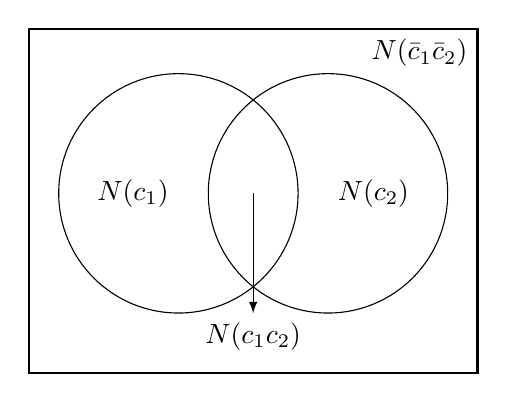
\begin{tikzpicture}[scale=0.95]
                \draw (-1,0) node[left] {$N(c_1)$} circle (1.6cm);
                \draw (1,0) node[right] {$N(c_2)$} circle (1.6cm);
                \draw[thick] (-3,-2.4) rectangle (3,2.2) node[below left] {$N(\bar{c}_1 \bar{c}_2)$};
                \draw[-latex] (0,0) -- (0,-1.6) node[below] {$N(c_1 c_2)$};
            \end{tikzpicture}
            \captionof{figure}{~\hspace{-2.75cm}~} \label{IAIAOAOAIJSJBJSKSI}
        \end{center}
    \end{minipage}
\end{myexample}

\newpage

\begin{myexample}
    Comenzamos con los mismos 100 estudiantes que en el ejemplo anterior y las mismas condiciones $c_1$, $c_2$, pero ahora consideramos una tercera condición, dada como sigue:
    \begin{align*}
        c_3 &: \text{ Un estudiante del IPN entre los 100 estudiantes de ingeniería y está inscrito en Programación.}
    \end{align*}
    Sigue siendo el caso que $N(c_1) = 35$, $N(c_2) = 30$ y $N(c_1 c_2) = 9$, pero ahora también se nos da que $N(c_3) = 30$, $N(c_1 c_3) = 11$, $N(c_2 c_3) = 10$ y $N(c_1 c_2 c_3) = 5$ (es decir, hay cinco de estos 100 estudiantes de primer año que están tomando Cálculo, Economía y Programación). Mirando la figura \ref{UAISISKKJJBJKOSPPIIW}, se sigue que
    $$N\left(\bar{c}_1 \bar{c}_2 \bar{c}_3\right) = N -\left[N\left(c_1\right) + N\left(c_2\right) + N\left(c_3\right)\right] + \left[N\left(c_1 c_2\right) + N\left(c_1 c_3\right) + N\left(c_2 c_3\right)\right] - N\left(c_1 c_2 c_3\right) .$$
    Entonces aquí tenemos
    $$N(\bar{c}_1 \bar{c}_2 \bar{c}_3) = 100 - [35 + 30 + 301 + 19 + 11 + 10] - 5 = 30.$$
    \begin{minipage}[l]{0.6\textwidth}
        Es decir, fuera de estos 100 alumnos, hay 30 que no están inscritos en ninguno de los cursos:
        \begin{tasks}[label=\roman*)](3)
            \task Cálculo
            \task Economía
            \task Programación
        \end{tasks}
        De manera análoga al ejemplo anterior,
        $$N (\bar{c}_3) = 70 = 100 - 30 = N - N(c_3),$$
        luego
        \begin{align*}
            N(\bar{c}_1 \bar{c}_3) = 46 & = 100 - [ 35 + 30] + 11 \\
            & = N - [N(c_1) + N(c_3)] + N(c_2 c_3),
        \end{align*}
        y por último,
        \begin{align*}
            N(\bar{c}_2 \bar{c}_3) = 50 & = 100 - [30 + 30] + 10 \\
            & = N - [N(c_2) + N(c_3)] + N(c_2 c_3).
        \end{align*}
    \end{minipage}~
    \begin{minipage}[r]{0.22\textwidth}
        \begin{center}
            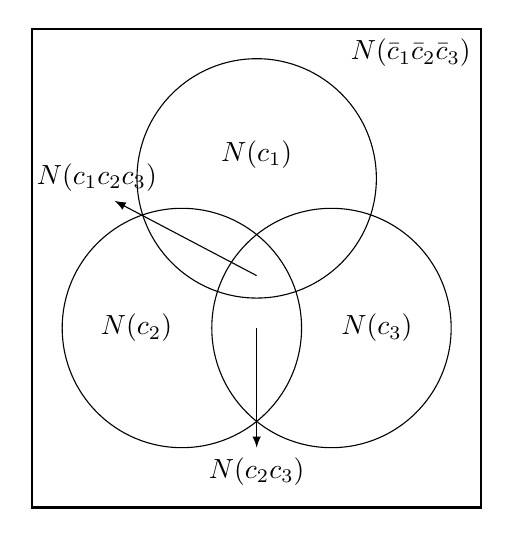
\begin{tikzpicture}[scale=0.95]
                \draw (-1,0) node[left] {$N(c_2)$} circle (1.6cm);
                \draw (1,0) node[right] {$N(c_3)$} circle (1.6cm);
                \draw (0,2) node[above] {$N(c_1)$} circle (1.6cm);
                \draw[thick] (-3,-2.4) rectangle (3,4) node[below left] {$N(\bar{c}_1 \bar{c}_2 \bar{c}_3)$};
                \draw[-latex] (0,0) -- (0,-1.6) node[below] {$N(c_2 c_3)$};
                \draw[-latex] (0,0.7) -- (-1.9,1.7) node[above] {$N(c_1 c_2 c_3) \quad\;$};
            \end{tikzpicture}
            \captionof{figure}{~\hspace{-2.75cm}~}\label{UAISISKKJJBJKOSPPIIW}
        \end{center}
    \end{minipage}
\end{myexample}

\begin{myexample}
    Con base en los resultados de los dos ejemplos anteriores, ahora para un conjunto finito $S$ (con $|S| = N$) y cuatro condiciones $c_1$, $c_2$, $c_3$, $c_4$ deberíamos tener
    \begin{equation}
        \begin{array}{rl}
            N \left( \bar{c}_1 \bar{c}_2 \bar{c}_3 \bar{c}_4 \right) = & \!\!\!\! N - \left[ N \left( c_1 \right) + N \left( c_2 \right) + N \left( c_3 \right) + N \left( c_4 \right) \right] + \left[ N \left( c_1 c_2 \right) + N\left( c_1 c_3 \right) \right. \\
            & \quad\quad \left. + N\left( c_1 c_4 \right) + N\left( c_2 c_3 \right) + N\left( c_2 c_4 \right) + N\left( c_3 c_4 \right) \right] - \left[ N \left( c_1 c_2 c_3 \right)  \right. \\
            & \quad\quad\quad\quad \left. + N \left( c_1 c_2 c_4 \right) + N \left( c_1 c_3 c_4 \right) + N \left( c_2 c_3 c_4 \right) \right] + N\left( c_1 c_2 c_3 c_4 \right) .
        \end{array} \label{JAIDJSJSKKLLOPS}
    \end{equation}
    Para demostrar que este es el caso, consideramos un elemento arbitrario $x$ de $S$ y demostramos que contó el mismo número de veces en ambos lados de la ecuación anterior.
    \begin{enumerate}[label=\arabic*)]
        \item[0)] Si $x$ no satisface ninguna de las cuatro condiciones, entonces se cuenta una vez en el lado izquierdo de la ecuación \eqref{JAIDJSJSKKLLOPS} [en $N\left(\bar{c}_1 \bar{c}_2 \bar{c}_3 \bar{c}_4\right)$], y una vez en el lado derecho de la ecuación \eqref{JAIDJSJSKKLLOPS} [en $N$].
        \item Si $x$ satisface solo una de las condiciones, digamos $c_1$, entonces no se cuenta en absoluto en el lado izquierdo de la ecuación \eqref{JAIDJSJSKKLLOPS}. Para el lado derecho de la ecuación \eqref{JAIDJSJSKKLLOPS}, $x$ se cuenta una vez en $N$ y una vez en $N\left(c_1\right)$, para un total de $1-1=0$ veces.
        \item Ahora supongamos que $x$ satisface las condiciones $c_2, c_4$ pero no satisface las condiciones $c_1$, $c_3$. Una vez más, $x$ no se cuenta en el lado izquierdo de la ecuación \eqref{JAIDJSJSKKLLOPS}. Para el lado derecho de la ecuación \eqref{JAIDJSJSKKLLOPS}, $x$ se cuenta una vez en $N$, una vez en cada uno de $N\left(c_2\right)$ y $N\left(c_4\right)$, y luego una vez en $N\left(c_2 c_4\right)$, se cuenta $\displaystyle 1-[1+1]+1=1-\binom{2}{1} + \binom{2}{2} = 0 $ veces.
        \item Continuando con el caso de tres condiciones, supondremos aquí que $x$ satisface las condiciones $c_1$, $c_2$ y $c_4$, pero no $c_3$. Como en los dos casos anteriores, $x$ no se cuenta en el lado izquierdo de la ecuación \eqref{JAIDJSJSKKLLOPS}. En el lado derecho de la ecuación \eqref{JAIDJSJSKKLLOPS}, $x$ se cuenta una vez en $N$, una vez en cada uno de $N\left(c_1\right)$, $N\left(c_2\right)$ y $N\left( c_4\right)$, una vez en cada uno de $N\left(c_1 c_2\right)$, $N\left(c_1 c_4\right)$ y $N\left(c_2 c_4\right)$ y, finalmente, una vez en $N\left(c_1 c_2 c_4\right)$. Así, en el lado derecho de la ecuación \eqref{JAIDJSJSKKLLOPS}, $x$ se cuenta $\displaystyle 1-[1+1+1]+[1+1+1]-1=1-\binom{3}{1} + \binom{3}{2} - \binom{3}{3} = 0$ veces, en total.
        \item Finalmente, si $x$ satisface las cuatro condiciones $c_1$, $c_2$, $c_3$, $c_4$, entonces una vez más no se cuenta en el lado izquierdo de la ecuación \eqref{JAIDJSJSKKLLOPS}. En el lado derecho de la ecuación \eqref{JAIDJSJSKKLLOPS}, $x$ se cuenta una vez para cada uno de los 16 términos en el lado derecho de esta ecuación para un total de $\displaystyle 1-[1+1+1+1]+[1+1+1+1+1 +1]-[1+1+1+1]+1=1- \binom{3}{1} + \binom{3}{2} - \binom{3}{3} = 0$ veces.

        En consecuencia, de estos cinco casos anteriores hemos demostrado que los dos lados de la ecuación \eqref{JAIDJSJSKKLLOPS} cuenta los mismos elementos de $S$, y esto proporciona una prueba combinatoria de la fórmula para $N(\bar{c}_1 \bar{c}_2 \bar{c}_3 \bar{c} _4)$.
    \end{enumerate}
    Ahora reconsideraremos la situación del ejemplo anterior e introduzcamos una cuarta condición como sigue:
    \begin{align*}
        c_4 &: \text{ Un estudiante del IPN entre los 100 estudiantes de ingeniería y está inscrito en Álgebra.}
    \end{align*}
    Ya sabemos que $N\left(c_1\right)=35$, $N\left(c_2\right)=30$, $N\left(c_3\right)=30$, $N\left(c_1 c_2\right)=9$, $N\left(c_1 c_3\right)=11$, $N\left(c_2 c_3\right)=10$ y $N\left(c_1 c_2 c_3\right)=5$. Si $N\left(c_4\right)=41$, $N\left(c_1 c_4\right)=13$, $N\left(c_2 c_4\right)=14$, $N\left(c_3 c_4\right)=10$, $N\left(c_1 c_2 c_4\right)=6$, $N\left(c_1 c_3 c_4\right)=6$, $N\left(c_2 c_3 c_4\right)=6$, y $N\left(c_1 c_2 c_3 c_4\right)=4$, entonces, usando la ecuación que se obtuvo arriba, se deduce que
    \begin{align*}
        N(\bar{c}_1 \bar{c}_2 \bar{c}_3 \bar{c}_4) & = 100-[35+30+30+41]+[9+11+13+10+14+10]-[5+6+6+6]+4 \\
        & = 100-136+67-23 +4=12.
    \end{align*}
    Así, de los 100 estudiantes del programa de primer año de ingeniería del IPN, hay 12 que no están tomando ninguno de los cuatro cursos: Cálculo, Economía, Programación y Álgebra.

    Si estamos interesados en el número (de estos 100 estudiantes) que están tomando Cálculo, pero ninguno de los otros tres cursos, entonces deberíamos querer calcular $N\left(c_1 \bar{c}_2 \bar{c} _3 \bar{c}_4\right)$. Para ello comenzamos observando que
    $$N(\bar{c}_2 \bar{c}_3 \bar{c}_4) = N(c_1 \bar{c}_2 \bar{c}_3 \bar{c}_4)+N(\bar{c}_1 \bar{c}_2 \bar{c}_3 \bar{c}_4),$$
    que puede establecerse mediante un argumento similar al anterior para $N\left(\bar{c}_1 \bar{c}_2 \bar{c}_3 \bar{c}_4\right)$. Esto nos lleva entonces a
    $$N\left(c_1 \bar{c}_2 \bar{c}_3 \bar{c}_4\right)=N\left(\bar{c_2} \bar{c}_3 \bar{c}_4\right)-N\left(\bar{c}_1 \bar{c}_2 \bar{c}_3 \bar{c}_4\right).$$
    Usando el resultado del ejemplo anterior encontramos que
    \begin{align*}
        N\left(\bar{c}_2 \bar{c}_3 \bar{c}_4\right) & = N-\left[N\left(c_2\right)+N\left(c_3\right)+ N\left(c_4\right)\right]+\left[N\left(c_2 c_3\right)+N\left(c_2 c_4\right)+N\left(c_3 c_4\right)\right] - N\left(c_2 c_3 c_4\right) \\
        &= 100-[30+30+41]+[10+14+10]-6=27,
    \end{align*}
    y
    $$N\left(c_1 \bar{c}_2 \bar{c}_3 \bar{c}_4\right)=N\left(\bar{c}_2 \bar{c}_3 \bar{c}_4 \right)-N\left(\bar{c}_1 \bar{c}_2 \bar{c}_3 \bar{c}_4\right)=27-12=15 .$$
    Entonces, hay 15 estudiantes en este grupo de 100 que están tomando Cálculo, pero ninguno de los otros cursos: Economía, Programación o Álgebra. Además, también observamos que
    \begin{align*}
        N\left(c_1 \bar{c}_2 \bar{c}_3 \bar{c}_4\right)& = N\left(\bar{c}_2 \bar{c}_3 \bar{c}_4\right)-N\left(\bar{c}_1 \bar{c}_2 \bar{c}_3 \bar{c}_4\right) \\
        & = \left\{N-\left[N\left(c_2\right)+N\left(c_3\right)+N\left(c_4\right)\right]+\left[N\left(c_2 c_3\right)+N\left(c_2 c_4\right)+N\left(c_3 c_4\right)\right]\right. \\
        & \quad \left.-N\left(c_2 c_3 c_4\right)\right\}-\left\{N-\left[N\left(c_1\right)+N\left(c_2\right)+N\left(c_3\right)+N\left(c_4\right)\right]\right. \\
        & \quad\quad +\left[N\left(c_1 c_2\right)+N\left(c_1 c_3\right)+N\left(c_1 c_4\right)+N\left(c_2 c_3\right)+N\left(c_2 c_4\right)+N\left(c_3 c_4\right)\right] \\
        & \quad\quad\quad \left.-\left[N\left(c_1 c_2 c_3\right)+N\left(c_1 c_2 c_4\right)+N\left(c_1 c_3 c_4\right)+N\left(c_2 c_3 c_4\right)\right]+N\left(c_1 c_2 c_3 c_4\right)\right\},
    \end{align*}
    o bien,
    \begin{align*}
        N\left(c_1 \bar{c}_2 \bar{c}_3 \bar{c}_4\right) & = N\left(c_1\right)-\left[N\left(c_1 c_2\right)+N\left(c_1 c_3\right)+N\left(c_1 c_4\right)\right] \\
        & +\left[N\left(c_1 c_2 c_3\right)+N\left(c_1 c_2 c_4\right)+N\left(c_1 c_3 c_4\right)\right]-N\left(c_1 c_2 c_3 c_4\right) .
    \end{align*}
    Entonces aquí $N\left(c_1 \bar{c}_2 \bar{c}_3 \bar{c}_4\right)=35-[9+11+13]+[5+6+6]-4= 35-33+17-4=15$, como encontramos arriba.
\end{myexample}

\noindent
\begin{minipage}[l]{0.6\textwidth}
    \hspace*{6mm}Habiendo visto los resultados de los ejemplos anteriores, ahora es el momento de generalizar estos resultados y establecer el principio de inclusión y exclusión. Sea $S$ un conjunto tal que $|S|=N$ y sean $c_1, \, c_2, \, \dots, \, c_t$ una colección de condiciones o propiedades satisfechas por algunos, o todos, los elementos de $S$. Algunos elementos de $S$ podrían satisfacer más de una de las condiciones, mientras que otros podrían no satisfacer ninguna. Para todo $1 \leq i \leq t$, $N\left(c_i\right)$ denota el número de elementos de $S$ que satisfacen la condición $c_i$ (los elementos de $S$ se cuentan cuando satisfacen solamente la condición $c_i$ y también cuando satisfacen $c_i$ y otras condiciones $c_j$, para $j \neq i$). Para cualesquiera $i$, $j \in \{ 1, \, 2, \, 3, \dots, \, t\}$, tales que $i \neq j$, $N\left(c_i c_j\right)$ denotará el número de elementos de $S$ que satisfacen ambas condiciones $c_i, c_j$ y tal vez otras más. Continuando de esta forma, si $1 \leq i, \, j, \, k \leq t$ son tres enteros distintos, entonces $N\left(c_i c_j c_k\right)$ denota el número de elementos de $S$ que satisfacen, tal vez entre otras, cada una de las condiciones $c_i$, $c_j$ y $c_k$.
    
    \hspace*{6mm}Para cada $1 \leq i \leq t$, $N\left(\bar{c}_i\right)=N-N\left(c_i\right)$ denota el número de elementos de $S$ que no satisfacen la condición $c_i$. Si $1 \leq i, \, j \leq t$, con $i \neq j$, $N\left(\bar{c}_i \bar{c}_j\right)$ denota el número de elementos de $S$ que no satisfacen alguna de las condiciones $c_i$ o $c_j$.

    \hspace*{6mm}Del diagrama de Venn de la figura \ref{ISISOOSOSOLSL}, vemos que $N\left(c_i\right)$ es el número de elementos del círculo del lado izquierdo y $N\left(c_j\right)$ es el número de elementos del círculo del lado derecho. Así, $N(\bar{c}_i \bar{c}_j)=N - \left[N\left(c_i\right)+N\left(c_j\right)\right]+N\left(c_i c_j\right)$ siendo $N\left(c_i c_j\right)$ los elementos de la intersección y $N\left(\bar{c}_i \bar{c}_j\right)$ los elementos que quedan fuera de la unión de estos círculos, donde se suma el último término debido a que fue eliminado dos veces en el término $\left[N\left(c_i\right)+N\left(c_j\right)\right]$.
\end{minipage}~
\begin{minipage}[r]{0.22\textwidth}
    \begin{center}
        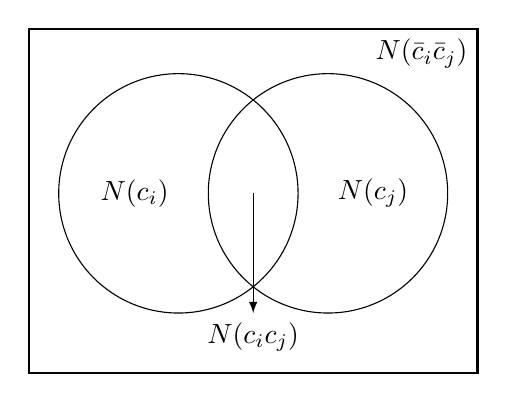
\begin{tikzpicture}[scale=0.95]
            \draw (-1,0) node[left] {$N(c_i)$} circle (1.6cm);
            \draw (1,0) node[right] {$N(c_j)$} circle (1.6cm);
            \draw[thick] (-3,-2.4) rectangle (3,2.2) node[below left] {$N(\bar{c}_i \bar{c}_j)$};
            \draw[-latex] (0,0) -- (0,-1.6) node[below] {$N(c_i c_j)$};
        \end{tikzpicture}
        \captionof{figure}{~\hspace{-2.75cm}~} \label{ISISOOSOSOLSL}

        \,\\

        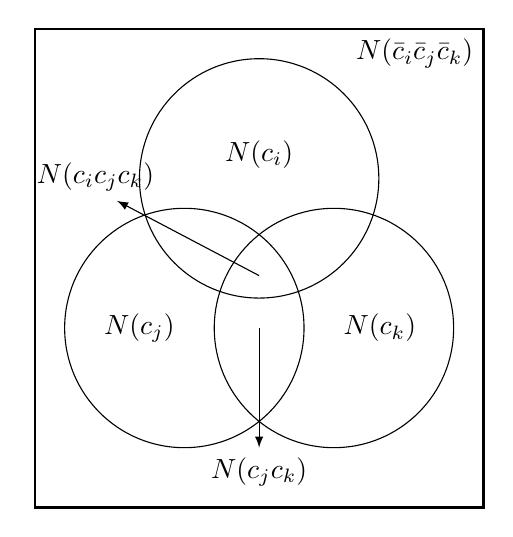
\begin{tikzpicture}[scale=0.95]
            \draw (-1,0) node[left] {$N(c_j)$} circle (1.6cm);
            \draw (1,0) node[right] {$N(c_k)$} circle (1.6cm);
            \draw (0,2) node[above] {$N(c_i)$} circle (1.6cm);
            \draw[thick] (-3,-2.4) rectangle (3,4) node[below left] {$N(\bar{c}_i \bar{c}_j \bar{c}_k)$};
            \draw[-latex] (0,0) -- (0,-1.6) node[below] {$N(c_j c_k)$};
            \draw[-latex] (0,0.7) -- (-1.9,1.7) node[above] {$N(c_i c_j c_k) \quad\;\;$};
        \end{tikzpicture}
        \captionof{figure}{~\hspace{-2.75cm}~}\label{ISIDODOODODODO}
    \end{center}
\end{minipage}

\newpage

De manera análoga, de la figura \ref{ISIDODOODODODO}, $N(c_i)$ es el número de elementos del círculo superior, $N(c_j)$ el número de elementos del círculo inferior izquierdo y $N(c_k)$ el número de elementos del círculo inferior derecho. Luego tenemos \\

%\begin{center}
    \noindent\begin{minipage}[l]{0.45\textwidth}
        \begin{center}
            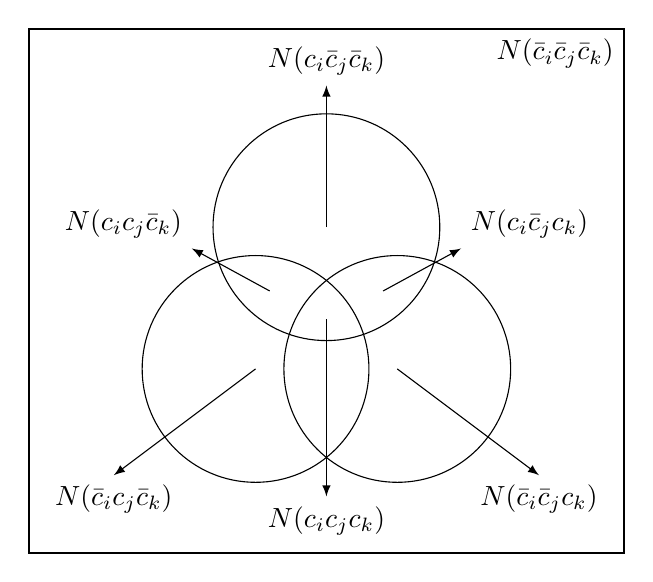
\begin{tikzpicture}[scale=0.9]
                \draw (-1,0) circle (1.6cm);
                \draw (1,0) circle (1.6cm);
                \draw (0,2) circle (1.6cm);
                \draw[thick] (-4.2,-2.6) rectangle (4.2,4.8) node[below left] {$N(\bar{c}_i \bar{c}_j \bar{c}_k)$};
                
                \draw[-latex] (0,0.7) -- (0,-1.8) node[below] {$N(c_i c_j c_k)$};
                
                \draw[-latex] (0.8,1.1) -- (1.9,1.7) node[above right] {$N(c_i \bar{c}_j c_k)$};
                
                \draw[-latex] (-0.8,1.1) -- (-1.9,1.7) node[above left] {$N(c_i c_j \bar{c}_k)$};
                
                \draw[-latex] (0,2) -- (0,4) node[above] {$N(c_i \bar{c}_j \bar{c}_k)$};
                
                \draw[-latex] (1,0) -- (3,-1.5) node[below] {$N(\bar{c}_i \bar{c}_j c_k)$};
                
                \draw[-latex] (-1,0) -- (-3,-1.5) node[below] {$N(\bar{c}_i c_j \bar{c}_k)$};
            \end{tikzpicture}
            \captionof{figure}{~\hspace{-1cm}~}\label{GHJJKKKHGTVJUHGG}
        \end{center}
    \end{minipage} \hspace{0.7cm}
    \begin{minipage}[l]{0.45\textwidth}
        \begin{center}
            \begin{tikzpicture}[thick,
            set/.style = {circle,
            minimum size = 3.2cm,
            fill=white}]
        
                \filldraw[SteelBlue1] (-3.7,-2.34) rectangle (3.7,4.32);
            
                % Set A
                \node[set] (A) at (1,0) {~};
                \node at (1,0) [right] {$N(c_k)$};
            
                % Set B
                \node[set] (B) at (-1,0) {~};
                \node at (-1,0) [left] {$N(c_j)$};
            
                % Set C
                \node[set] (C) at (0,2) {~};
                \node at (0,2) [above] {$N(c_i)$};
            
                % Intersection
                \begin{scope}
                    \clip (-1,0) circle (1.6cm);
                    \clip (1,0) circle (1.6cm);
                    \clip (0,2) circle (1.6cm);
                    \fill[SteelBlue1] (0,0) circle (1.6cm);
                \end{scope}
            
                % Circles outline
                \draw (-1,0) circle (1.6cm);
                \draw (1,0) circle (1.6cm);
                \draw (0,2) circle (1.6cm);
            
                \draw[thick] (-3.7,-2.34) rectangle (3.7,4.32) node[below left,fill=white] {$N(\bar{c}_i \bar{c}_j \bar{c}_k)$};
            
                \draw[-latex] (0,0.7) -- (1.9,1.7) node[above right,fill=white] {$N(c_i c_j c_k)$};
            \end{tikzpicture}
            \captionof{figure}{~\hspace{-1cm}~}\label{IAKANKKNNAOOOUAUA}
        \end{center}
    \end{minipage}
%\end{center}

\,\\
\noindent
De la figura \ref{GHJJKKKHGTVJUHGG}, obtenemos que
\begin{equation}
    {\extrarowheight = -0.5ex
    \renewcommand{\arraystretch}{1.5}
    \begin{array}{rl}
        N(c_i) = & \!\!\!\! N(c_i \bar{c}_j \bar{c}_k) + N(c_i c_j \bar{c}_k) + N(c_i \bar{c}_j c_k) + N(c_i c_j c_k), \\
        N(c_j) = & \!\!\!\! N(\bar{c}_i c_j \bar{c}_k) + N(c_i c_j \bar{c}_k) + N(\bar{c}_i c_j c_k) + N(c_i c_j c_k), \\
        N(c_k) = & \!\!\!\! N(\bar{c}_i \bar{c}_j c_k) + N(c_i \bar{c}_j c_k) + N(\bar{c}_i c_j c_k) + N(c_i c_j c_k).
    \end{array} } \label{JSJSJSJSKKLOIUWU}
\end{equation}
Asimismo,
\begin{equation}
    {\extrarowheight = -0.5ex
    \renewcommand{\arraystretch}{1.5}
    \begin{array}{rl}
        N(c_i c_j) = & \!\!\!\! N(c_i c_j \bar{c}_k) + N(c_i c_j c_k), \\
        N(c_i c_k) = & \!\!\!\! N(c_i \bar{c}_j c_k) + N(c_i c_j c_k), \\
        N(c_j c_k) = & \!\!\!\! N(\bar{c}_i c_j c_k) + N(c_i c_j c_k).
    \end{array} } \label{JAJAKNNIIUWYBNNWUWYWHJI}
\end{equation}
Multiplicando por $-1$ las expresiones de \eqref{JSJSJSJSKKLOIUWU}, se sigue que
\begin{equation}
    {\extrarowheight = -0.5ex
    \renewcommand{\arraystretch}{1.5}
    \begin{array}{rl}
        -N(c_i) = & \!\!\!\! -N(c_i \bar{c}_j \bar{c}_k) - N(c_i c_j \bar{c}_k) - N(c_i \bar{c}_j c_k) - N(c_i c_j c_k), \\
        -N(c_j) = & \!\!\!\! -N(\bar{c}_i c_j \bar{c}_k) - N(c_i c_j \bar{c}_k) - N(\bar{c}_i c_j c_k) - N(c_i c_j c_k), \\
        -N(c_k) = & \!\!\!\! -N(\bar{c}_i \bar{c}_j c_k) - N(c_i \bar{c}_j c_k) - N(\bar{c}_i c_j c_k) - N(c_i c_j c_k).
    \end{array} } \label{JAIALAOOAUQYABNKQKQK}
\end{equation}
De las expresiones \eqref{JAIALAOOAUQYABNKQKQK} y \eqref{JAJAKNNIIUWYBNNWUWYWHJI}, se sigue que
\begin{align*}
    N(\bar{c}_i \bar{c}_j \bar{c}_k) + N(c_i c_j c_k) & = N - N(c_i) - N(c_j) - N(c_k) + N(c_i c_j) + N(c_i c_k) + N(c_j c_k) \\
    & = N - N(c_i \bar{c}_j \bar{c}_k) - N(c_i c_j \bar{c}_k) - N(c_i \bar{c}_j c_k) - N(c_i c_j c_k) -N(\bar{c}_i c_j \bar{c}_k) - N(c_i c_j \bar{c}_k) \\
    & \quad - N(\bar{c}_i c_j c_k) - N(c_i c_j c_k) - N(\bar{c}_i \bar{c}_j c_k) - N(c_i \bar{c}_j c_k) - N(\bar{c}_i c_j c_k) - N(c_i c_j c_k) \\
    & \quad + N(c_i c_j \bar{c}_k) + N(c_i c_j c_k) + N(c_i \bar{c}_j c_k) + N(c_i c_j c_k) + N(\bar{c}_i c_j c_k) + N(c_i c_j c_k).
\end{align*}
Simplificando, se obtiene que (vea la figura \ref{IAKANKKNNAOOOUAUA})
$$N - [N(c_i c_j \bar{c}_k) + N(c_i \bar{c}_j c_k) + N(\bar{c}_i c_j c_k) + N(c_i \bar{c}_j \bar{c}_j) + N(\bar{c}_i c_j \bar{c}_k) + N(\bar{c}_i \bar{c}_j c_j)] = N(\bar{c}_i \bar{c}_j \bar{c}_k) + N(c_i c_j c_k).$$
Probando y obteniendo así,
$$
N\left(\bar{c}_i \bar{c}_j \bar{c}_k\right) = N -\left[N\left(c_i\right) + N\left(c_j\right) + N\left(c_k\right)\right] + \left[N\left(c_i c_j\right) + N\left(c_i c_k\right) + N\left(c_j c_k\right)\right] - N\left(c_i c_j c_k\right) .
$$

Con los preliminares antes vistos, enunciamos el siguiente teorema.

\newpage

\begin{theorem}{El principio de inclusión y exclusión [PIE]}{}
    Consideremos un conjunto $S$ tal que $|S|=N$ y las condiciones $c_i$, $1 \leq i \leq t$ satisfechas por algunos de los elementos de $S$. El número de elementos de $S$ que no satisfacen ninguna de las condiciones $c_i$, $1 \leq i \leq t$, se denota con $\overline{N}=N\left(\bar{c}_1 \bar{c}_2 \bar{c}_3 \dots \bar{c}_t\right)$, donde
    \begin{align*}
        \overline{N} & = N-\left[N\left(c_1\right)+N\left(c_2\right)+N\left(c_3\right)+\cdots+N\left(c_t\right)\right] \\
        & \quad\quad\quad +\left[N\left(c_1 c_2\right)+N\left(c_1 c_3\right)+\cdots+N\left(c_1 c_t\right)+N\left(c_2 c_3\right)+\cdots+N\left(c_{t-1} c_t\right)\right] \\
        & \quad\quad\quad\quad -\left[N\left(c_1 c_2 c_3\right)+N\left(c_1 c_2 c_4\right)+\cdots+N\left(c_1 c_2 c_t\right)+N\left(c_1 c_3 c_4\right)+\cdots\right. \\
        & \quad\quad\quad\quad\quad  \left.+N\left(c_1 c_3 c_t\right)+\cdots+N\left(c_{t-2} c_{t-1} c_t\right)\right]+\cdots+(-1)^t N\left(c_1 c_2 c_3 \ldots c_t\right),
    \end{align*}
    o bien
    \begin{equation}
        \overline{N} = N-\sum_{1 \leq i \leq t} N\left(c_i\right)+\sum_{1 \leq i<j \leq t} N\left(c_i c_j\right)-\sum_{1 \leq i<j<k \leq t} N\left(c_i c_j c_k\right)+\cdots +(-1)^t N\left(c_1 c_2 c_3 \dots c_t\right). \label{JAISKKANNJSISJSJ}
    \end{equation}

    \tcblower
    \textbf{\color{jblueleft}Demostración:} Establezcamos y demostremos este resultado mediante inducción sobre $t$. Así,
    \begin{enumerate}[label=\roman*)]
        \item Si $t = 1$, entonces
        $$S = \left\{x \in S \mid x \text{ satisface } c_1 \right\} \cup \left\{x \in S \mid x \text{ no satisface } c_1 \right\}$$
        y esta es obviamente una unión disjunta. Luego, por el principio de suma, se deduce que
        $$N = N(c_1) + \overline{N} \Longrightarrow \overline{N} = N - N(c_1).$$
        Por tanto, PIE se cumple para $t = 1$.
        \item Supongamos que el PIE se cumple para algunas $t \in \NN$. Vamos a demostrarlo para $t + 1$.

        Para $i \in \{ 1, \, 2, \, \dots, \, t + 1 \}$, sea $S_i := \left\{ x \in S \mid x \text{ satisface } c_i \right\}$. Entonces, asumiendo que PIE se mantiene para $t$, tenemos que
        $$\left| (S \backslash S_{t+1}) \backslash \left( \bigcup_{i=1}^{t} S_i \right) \right| = |S \backslash S_{t+1}| + \sum_{I \subseteq \{1, \, \dots, \, t \} } (-1)^{|I|} \left| \bigcap_{i \in I} \big(S_i \cap (S \backslash S_{t+1}) \big) \right| .$$
        Eso implica que
        \begin{align*}
            \left| S \backslash \left( \bigcup_{i=1}^{t+1} S_i \right) \right| & = \left|(S \backslash S_{t+1}) \backslash \left( \bigcup_{i=1}^{t} S_i \right) \right| \\
            & = |S \backslash S_{t+1}| + \sum_{I \subseteq \{1, \, \dots, \, t \} } (-1)^{|I|} \left| \bigcap_{i \in I} \big(S_i \cap (S \backslash S_{t+1}) \big) \right| \\
            & = |S| - |S_{t+1}| + \sum_{I \subseteq \{1, \, \dots, \, t \} } (-1)^{|I|} \left( \left| \bigcap_{i \in I} S_i \right| - \left| \bigcap_{i \in I} (S_i \cap S_{t+1}) \right| \right) \\
            & = |S| - |S_{t+1}| + \sum_{I \subseteq \{1, \, \dots, \, t \} } (-1)^{|I|} \left| \bigcap_{i \in I} S_i \right| + \sum_{I \subseteq \{ 1, \, \dots, \, t \} } (-1)^{|I| + 1} \left| \bigcap_{i \in I \cup \{ t + 1 \} } S_i \right| \\
            & = |S| + \sum_{I \subseteq \{ 1, \, \dots, \, t+1 \} } (-1)^{|I|} \left| \bigcap_{i \in I} S_i \right|
        \end{align*}
        y esto es exactamente PIE para $t + 1$, ya que
        $$N = \left| S \backslash \left( \bigcup_{i=1}^{t+1} S_i \right) \right|$$
        y
        $$N(c_{i_1} c_{i_2} \dots c_{i_k}) = \left| \bigcup_{i \in I} S_i \right|$$
        donde $I = \{ i_1, \, \dots, \, i_k \} \subseteq \{ 1, \, \dots, \, t + 1 \}$.
    \end{enumerate}
    Por el principio de inducción matemática, PIE se cumple para toda $t \in \NN$. Así, si
    $$S_i := \left\{ x \in S \mid x \text{ satisface } c_i \right\}$$
    entonces
    $$S \backslash \left( \bigcup_{i=1}^{t+1} S_i \right)= (S \backslash S_{t+1}) \backslash \left( \bigcup_{i=1}^{t} S_i \right).$$
    
    Si aún no queda claro, daremos una demostración combinatoria. El argumento recordará las ideas que vimos en el último ejemplo al establecer la fórmula para $N(\bar{c}_1 \bar{c}_2 \bar{c}_3 \bar{c}_4)$.
    
    \hspace*{6mm}Para cada $x \in S$ demostramos que x contribuye con el mismo recuento, ya sea 0 o 1, a cada lado de la ecuación \eqref{JAISKKANNJSISJSJ}.
    
    \hspace*{6mm}Si $x$ no satisface ninguna de las condiciones, entonces x se cuenta una vez en $\overline{N}$ y una vez en $N$, pero no en ninguno de los otros términos de la ecuación \eqref{JAISKKANNJSISJSJ}. En consecuencia, $x$ aporta un conteo de 1 a cada lado de la ecuación.
    
    \hspace*{6mm}La otra posibilidad es que $x$ satisfaga exactamente $r$ de las condiciones donde $1 \leq r \leq t$. En este caso $x$ no aporta nada a $\overline{N}$. Pero en el lado derecho de la ecuación \eqref{JAISKKANNJSISJSJ}, se cuenta $x$.
    \begin{enumerate}[label=\arabic*)]
        \item Una vez en $N$.
        \item $r$ veces en $\displaystyle \sum_{1 \leq i \leq t} N(c_i)$ (una vez para cada una de las condiciones $r$).
        \item $\displaystyle \binom{r}{2}$ veces en $\displaystyle \sum_{1 \leq i < j \leq t} N(c_i c_j)$ (una vez por cada par de condiciones seleccionadas de las $r$ condiciones que satisface).
        \item $\displaystyle \binom{r}{3}$ veces en $\displaystyle \sum_{1 \leq i < j < k \leq t} N(c_i c_j c_k)$.

        \,\\
        \begin{tikzpicture}
            \draw[dash pattern=on \pgflinewidth off 2pt,thick] (0,0) -- (6,0);
        \end{tikzpicture}
        \,\\
        
        \item[$r + 1)$] $\displaystyle \binom{r}{r} = 1$ vez en $\displaystyle \sum N(c_{i_1} c_{i_2} \dots c_{i_r})$, donde la suma se toma de todas las selecciones de tamaño $r$ de las condiciones $t$.
    \end{enumerate}
    En consecuencia, en el lado derecho de la ecuación \eqref{JAISKKANNJSISJSJ}, se cuenta $x$
    $$1 - r + \binom{r}{2} - \binom{r}{3} \pm \cdots + (-1)^r \binom{r}{r} = [1 + (-1)]^r = 0^r = 0 \text{ veces},$$
    por el teorema del binomio. Por tanto, los dos lados de la ecuación \eqref{JAISKKANNJSISJSJ} cuenta los mismos elementos de $S$ y se verifica la igualdad.
\end{theorem}

\newpage

\begin{corollary}
    Según las hipótesis del teorema anterior, el número de elementos de $S$ que satisfacen al menos una de las condiciones $c_i$, donde $1 \leq i \leq t$, está dado por $N(c_1 \text{ ó } c_2 \text{ ó } \dots \text{ ó } c_t) = N - \overline{N}$.
\end{corollary}

\begin{myexample}
    ¿De cuántas formas pueden permutarse las 26 letras del alfabeto de tal manera que ninguno de los patrones sea \textit{car}, \textit{dog}, \textit{pun}, o \textit{byte}?

    \tcblower
    \textbf{\color{jblueleft}Solución:} Mostremos algunas permutaciones:
    $$\begin{array}{l}
        \bm{\textcolor{jblueleft}{car}}dfghijlmno\bm{\textcolor{jblueleft}{byte}}pqsukvwxz \\
        dfghijl\bm{\textcolor{jblueleft}{car}}mnopqsukv\bm{\textcolor{jblueleft}{byte}}wxz \\
        b\bm{\textcolor{jblueleft}{car}}efhijlm\bm{\textcolor{jblueleft}{dog}}qst\bm{\textcolor{jblueleft}{pun}}kvwxyz \\
        b\bm{\textcolor{jblueleft}{car}}efhijlmqst\bm{\textcolor{jblueleft}{pun}}kv\bm{\textcolor{jblueleft}{dog}}wxyz
    \end{array}$$
    Sea $S$ el conjunto de todas las permutaciones de 26 letras. Entonces $|S|=26!$. Para todo $1 \leq i \leq 4$, una permutación de, $S$ satisface la condición $c_i$ si la permutación contiene \textit{car}, \textit{dog}, \textit{pun} o \textit{byte}, respectivamente.
    
    Para calcular $N\left(c_i\right)$, por ejemplo, contamos el número de formas en que pueden permutarse los 24 símbolos \textit{car}, $b, \, d, \, e, \, f, \, \dots, \, p, \, q, \, s, \, t, \, \dots, \, x, \, y, \, z$. Así, $N\left(c_1\right)=24!$ y de una manera similar obtenemos
    $$N\left(c_2\right)=N\left(c_3\right)=24 !, \quad \text { mientras que } N\left(c_4\right)=23 !$$
    Para $N\left(c_1 c_2\right)$, trabajamos con los 22 símbolos \textit{car}, \textit{dog}, $b, e, f, h, i, \ldots, m, n, p, q, s, t, \ldots$, $x, y, z$, que pueden permutarse de $22!$ formas. De aquí obtenemos que $N\left(c_1 c_2\right)=22!$ y con otros cálculos semejantes obtenemos
    $$N\left(c_1 c_3\right)=N\left(c_2 c_3\right)=22 !, \quad N\left(c_i c_4\right)=21 !, i \neq 4 .$$
    Además,
    $$N\left(c_1 c_2 c_3\right)=20 !, \quad N\left(c_i c_j c_4\right)=19 !, \quad 1 \leq i<j \leq 3, \quad  \text{ y } N\left(c_1 c_2 c_3 c_4\right) = 17!$$
    Así, el número de permutaciones de $S$ que no contienen ninguno de los patrones dados es
    \begin{align*}
        N\left(\bar{c}_1 \bar{c}_2 \bar{c}_3 \bar{c}_4\right) & = 26 !-[3(24 !)+23 !]+[3(22 !)+3(21) !]-[20 !+3(19) !]+17. \\
        & = 401 \, 407 \, 786 \, 381 \, 839 \, 570 \, 837 \, 504 \, 017.
    \end{align*}
\end{myexample}

\begin{myexample}
    Para $n \in \ZZ[+]$, $n \geq 2$, sea $\phi(n)$ el número de enteros positivos $m$, tales que $1 \leq m<n$ y $\operatorname{mcd}(m, \, n) = 1$, esto es, $m$, $n$ son primos relativos. Esta función es la función phi de Euler y surge en varias situaciones del álgebra abstracta relacionadas con la enumeración. Encontramos que $\phi(2)=1$, $\phi(3)=2$, $\phi(4)=2$, $\phi(5)=4$ y $\phi(6)=2$. Para cualquier primo $p$, $\phi(p) = p-1$. Queremos obtener una fórmula para $\phi(n)$ relacionada con $n$ para no tener que hacer una comparación caso por caso para todo $m$, $1 \leq m < n$, con el entero $n$.
    
    La deducción de nuestra fórmula usará el principio de inclusión y exclusión. Procedemos como sigue: para $n \geq 2$, usamos el teorema fundamental de la aritmética y escribimos $p_1^{e_1} p_2^{e_2} \cdots p_t^{e_t}$, donde $p_1, \, p_2, \, \dots, \, p_t$ son primos distintos y $e_i \geq 1$, para todo $1 \leq i \leq t$. Consideremos el caso en que $t=4$. Esto será suficiente para demostrar la idea general.
    
    Si $S=\{1, \, 2, \, 3, \dots, \, n\}$, tenemos $N = |S|$ y para todo $1 \leq i \leq 4$, decimos que $k \in S$ satisface la condición $c_i$ si $k$ es divisible entre $p_i$. Para $1 \leq k < n, \operatorname{mcd}(k, \, n) = 1$ si $k$ no es divisible entre cualquiera de los primos $p_i$, donde $1 \leq i \leq 4$. Por lo tanto $\phi(n) = N\left(\bar{c}_1 \bar{c}_2 \bar{c}_3 \bar{c}_4\right)$.
    
    Para todo $1 \leq i \leq 4$, tenemos $N\left(c_i\right)=n / p_i$; $N\left(c_i c_j\right)=n /\left(p_i p_j\right)$, para todo $1 \leq i<j \leq 4$. También, $N\left(c_i c_j c_{\ell}\right)=n /\left(p_i p_j p_{\ell}\right)$, para todos $1 \leq i<j<\ell \leq 4$, y $N\left(c_1 c_2 c_3 c_4\right)=n /\left(p_1 p_2 p_3 p_4\right)$. Así,
    \begin{align*}
        \phi(n) & = S_0-S_1+S_2-S_3+S_4 \\
        & = n-\left[\frac{n}{p_1}+\cdots+\frac{n}{p_4}\right]+\left[\frac{n}{p_1 p_2}+\frac{n}{p_1 p_3}+\cdots+\frac{n}{p_3 p_4}\right] \\
        & \hspace{5cm} -\left[\frac{n}{p_1 p_2 p_3}+\cdots+\frac{n}{p_2 p_3 p_4}\right]+\frac{n}{p_1 p_2 p_3 p_4} \\
        & = n\left[1-\left(\frac{1}{p_1}+\cdots+\frac{1}{p_4}\right)+\left(\frac{1}{p_1 p_2}+\frac{1}{p_1 p_3}+\cdots+\frac{1}{p_3 p_4}\right)\right. \\
        & \hspace{5cm} \left.-\left(\frac{1}{p_1 p_2 p_3}+\cdots+\frac{1}{p_2 p_3 p_4}\right)+\frac{1}{p_1 p_2 p_3 p_4}\right] \\
        & = \frac{n}{p_1 p_2 p_3 p_4}\left[p_1 p_2 p_3 p_4-\left(p_2 p_3 p_4+p_1 p_3 p_4+p_1 p_2 p_4+p_1 p_2 p_3\right) \right. \\
        & \hspace{5cm} + \left(p_3 p_4+p_2 p_4+p_2 p_3+p_1 p_4+p_1 p_3+p_1 p_2\right) \\
        & \hspace{5cm} - (p_4 + p_3 + p_2 + p_1) + 1] \\
        & = \frac{n}{p_1 p_2 p_3 p_4}\left[ (p_1 - 1)(p_2 -1)(p_3 - 1)(p_4 - 1)\right]. \\
        & = n\left[\frac{p_1-1}{p_1} \cdot \frac{p_2-1}{p_2} \cdot \frac{p_3-1}{p_3} \cdot \frac{p_4-1}{p_4}\right]=n \prod_{i=1}^4\left(1-\frac{1}{p_i}\right) .
    \end{align*}
    En general, $\displaystyle \phi(n)=n \prod_{p \, \mid \, n}\left(1-\frac{1}{p}\right)$, donde el producto se toma sobre todos los primos $p$ que dividen a $n$. Cuando $n=p$, un primo, $\displaystyle \phi(n)=\phi(p)=p\left(1-\frac{1}{p}\right)=p-1$, como observamos antes. Para $n=23 \, 100$ encontramos que
    \begin{align*}
        \phi(23 \, 100) & =\phi\left(2^2 \cdot 3 \cdot 5^2 \cdot 7 \cdot 11\right) \\
        & = (23 \, 100)\left(1-\frac{1}{2}\right)\left(1-\frac{1}{3}\right)\left(1-\frac{1}{5}\right)\left(1-\frac{1}{7}\right)\left(1-\frac{1}{11}\right) \\
        & =4 \, 800.
    \end{align*}
\end{myexample}

\section{Generalizaciones del principio}

Consideremos un conjunto $S$ con $|S|=N$ y condiciones $c_1, \, c_2, \, \dots, \, c_t$ satisfechas por alguno de los elementos de $S$. En la sección anterior vimos cómo la inclusión y exclusión nos proporcionan una manera de determinar $N\left(\bar{c}_1 \bar{c}_2 \dots \bar{c}_t\right)$, el número de elementos de $S$ que no satisfacen ninguna de las $t$ condiciones. Si $m \in \mathbb{Z}^{+}$ y $1 \leq m \leq t$, queremos determinar ahora $E_m$, el número de elementos de $S$ que satisfacen exactamente $m$ de las $t$ condiciones (ahora podemos obtener $E_0$). Podemos escribir ecuaciones como
$$E_1=N\left(c_1 \bar{c}_2 \bar{c}_3 \dots \bar{c}_t\right)+N\left(\bar{c}_1 c_2 \bar{c}_3 \dots \bar{c}_t\right)+\cdots+N\left(\bar{c}_1 \bar{c}_2 \bar{c}_3 \dots \bar{c}_{t-1} c_t\right),$$
y
$$E_2=N\left(c_1 c_2 \bar{c}_3 \dots \bar{c}_t\right)+N\left(c_1 \bar{c}_2 c_3 \dots \bar{c}_t\right)+\cdots+N\left(\bar{c}_1 \bar{c}_2 \bar{c}_3 \dots \bar{c}_{t-2} c_{t-1} c_t\right)$$
y aunque estos resultados no nos ayudan tanto como quisiéramos, serán un punto de partida útil cuando examinemos los diagramas de Venn para los casos $t=3$ y 4.

En la figura \ref{JAJAJAJJTTTVVGTS}, donde $t=3$, colocamos una condición numerada al lado del círculo que representa los elementos de $S$ que satisfacen una condición particular. Entonces $E_1$ es igual al número de elementos en las regiones 2, 3 y 4. Pero también podemos escribir
$$E_1=N\left(c_1\right)+N\left(c_2\right)+N\left(c_3\right)-2\left[N\left(c_1 c_2\right)+N\left(c_1 c_3\right)+N\left(c_2 c_3\right)\right]+3 N\left(c_1 c_2 c_3\right).$$

En $N\left(c_1\right)+N\left(c_2\right)+N\left(c_3\right)$ contamos los elementos de las regiones 5, 6 y 7 dos veces y los de la región 8 tres veces. En el siguiente término, los elementos de las regiones 5, 6 y 7 se eliminan dos veces. Quitamos los elementos de la región 8 seis veces en $2\left[N\left(c_1 c_2\right)+\right.$ $N\left(c_1 c_3\right)+N\left(c_2 c_3\right)$], y después los añadimos en el término $3 N\left(c_1 c_2 c_3\right)$; por último, no contamos ninguno de los elementos de la región 8. Por lo tanto, tenemos $\displaystyle E_1=S_1-2 S_2+3 S_3=S_1 - \binom{2}{1}S_2 + \binom{3}{2}S_3$.

\begin{figure}[h!]
    \centering
    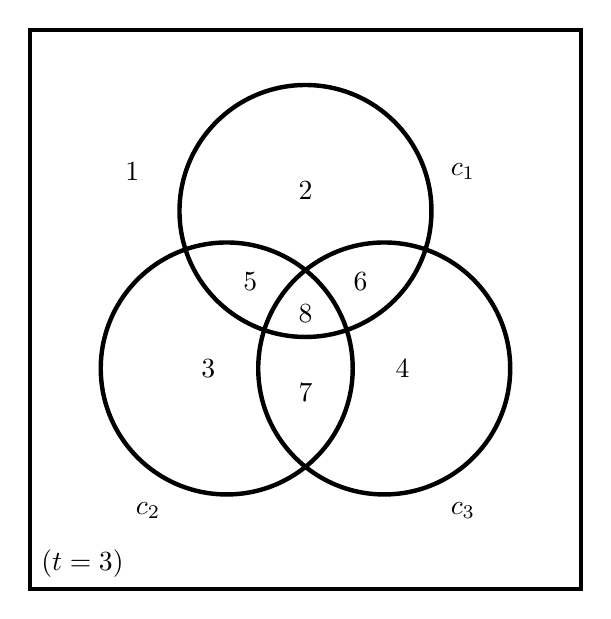
\begin{tikzpicture}
        \draw[ultra thick] (-1,0) node[left] {$3$} circle (1.6cm);
        \draw[ultra thick] (1,0) node[right] {$4$} circle (1.6cm);
        \draw[ultra thick] (0,2) node[above] {$2$} circle (1.6cm);
        \draw[ultra thick] (-3.5,-2.8) node[above right] {$(t = 3)$} rectangle (3.5,4.3);
        \node at (0,-0.3) {$7$};
        \node at (0,0.7) {$8$};
        \node at (-0.7,1.1) {$5$};
        \node at (0.7,1.1) {$6$};
        \node at (-2.2,2.5) {$1$};
        \node at (-2,-1.8) {$c_2$};
        \node at (2,-1.8) {$c_3$};
        \node at (2,2.5) {$c_1$};
    \end{tikzpicture}
    \caption{~}\label{JAJAJAJJTTTVVGTS}
\end{figure}

En el caso de $E_2$, nuestra ecuación anterior indica que queremos contar los elementos de $S$ en las regiones 5, 6 y 7. Del diagrama de Venn,
$$E_2=N\left(c_1 c_2\right)+N\left(c_1 c_3\right)+N\left(c_2 c_3\right)-3 N\left(c_1 c_2 c_3\right)=S_2-3 S_3=S_2-\binom{3}{1} S_3,$$
y
$$E_3=N\left(c_1 c_2 c_3\right)=S_3$$

En la figura \ref{UAJSBSNZSKKS}, las condiciones $c_1$, $c_2$, $c_3$ están asociadas con subconjuntos circulares de $S$, mientras que $c_4$ está asociada con el área de forma bastante irregular constituida por las regiones 4, 8, 9, 11, 12, 13, 14 y 16. Para cada $1 \leq i \leq 4$, $E_i$ está determinada como sigue:
\begin{itemize}
    \item $E_1$ [regiones 2, 3, 4, 5]:
    \begin{align*}
        E_1 & = \left[N\left(c_1\right) + N\left(c_2\right) + N\left(c_3\right) + N\left(c_4\right)\right]  \\
        & \quad -2\left[N\left(c_1 c_2\right)+N\left(c_1 c_3\right)+N\left(c_1 c_4\right)+N\left(c_2 c_3\right)+N\left(c_2 c_4\right)+N\left(c_3 c_4\right)\right] \\
        & \quad +3\left[N\left(c_1 c_2 c_3\right)+N\left(c_1 c_2 c_4\right)+N\left(c_1 c_3 c_4\right)+N\left(c_2 c_3 c_4\right)\right] - 4 N\left(c_1 c_2 c_3 c_4\right) \\
        & = S_1-2 S_2+3 S_3-4 S_4 =S_1-\binom{2}{1} S_2 + \binom{3}{2} S_3-\binom{4}{3} S_4 .
    \end{align*}
    
    \begin{figure}[h!]
    \centering
    \begin{tikzpicture}
        \node at (0,0) {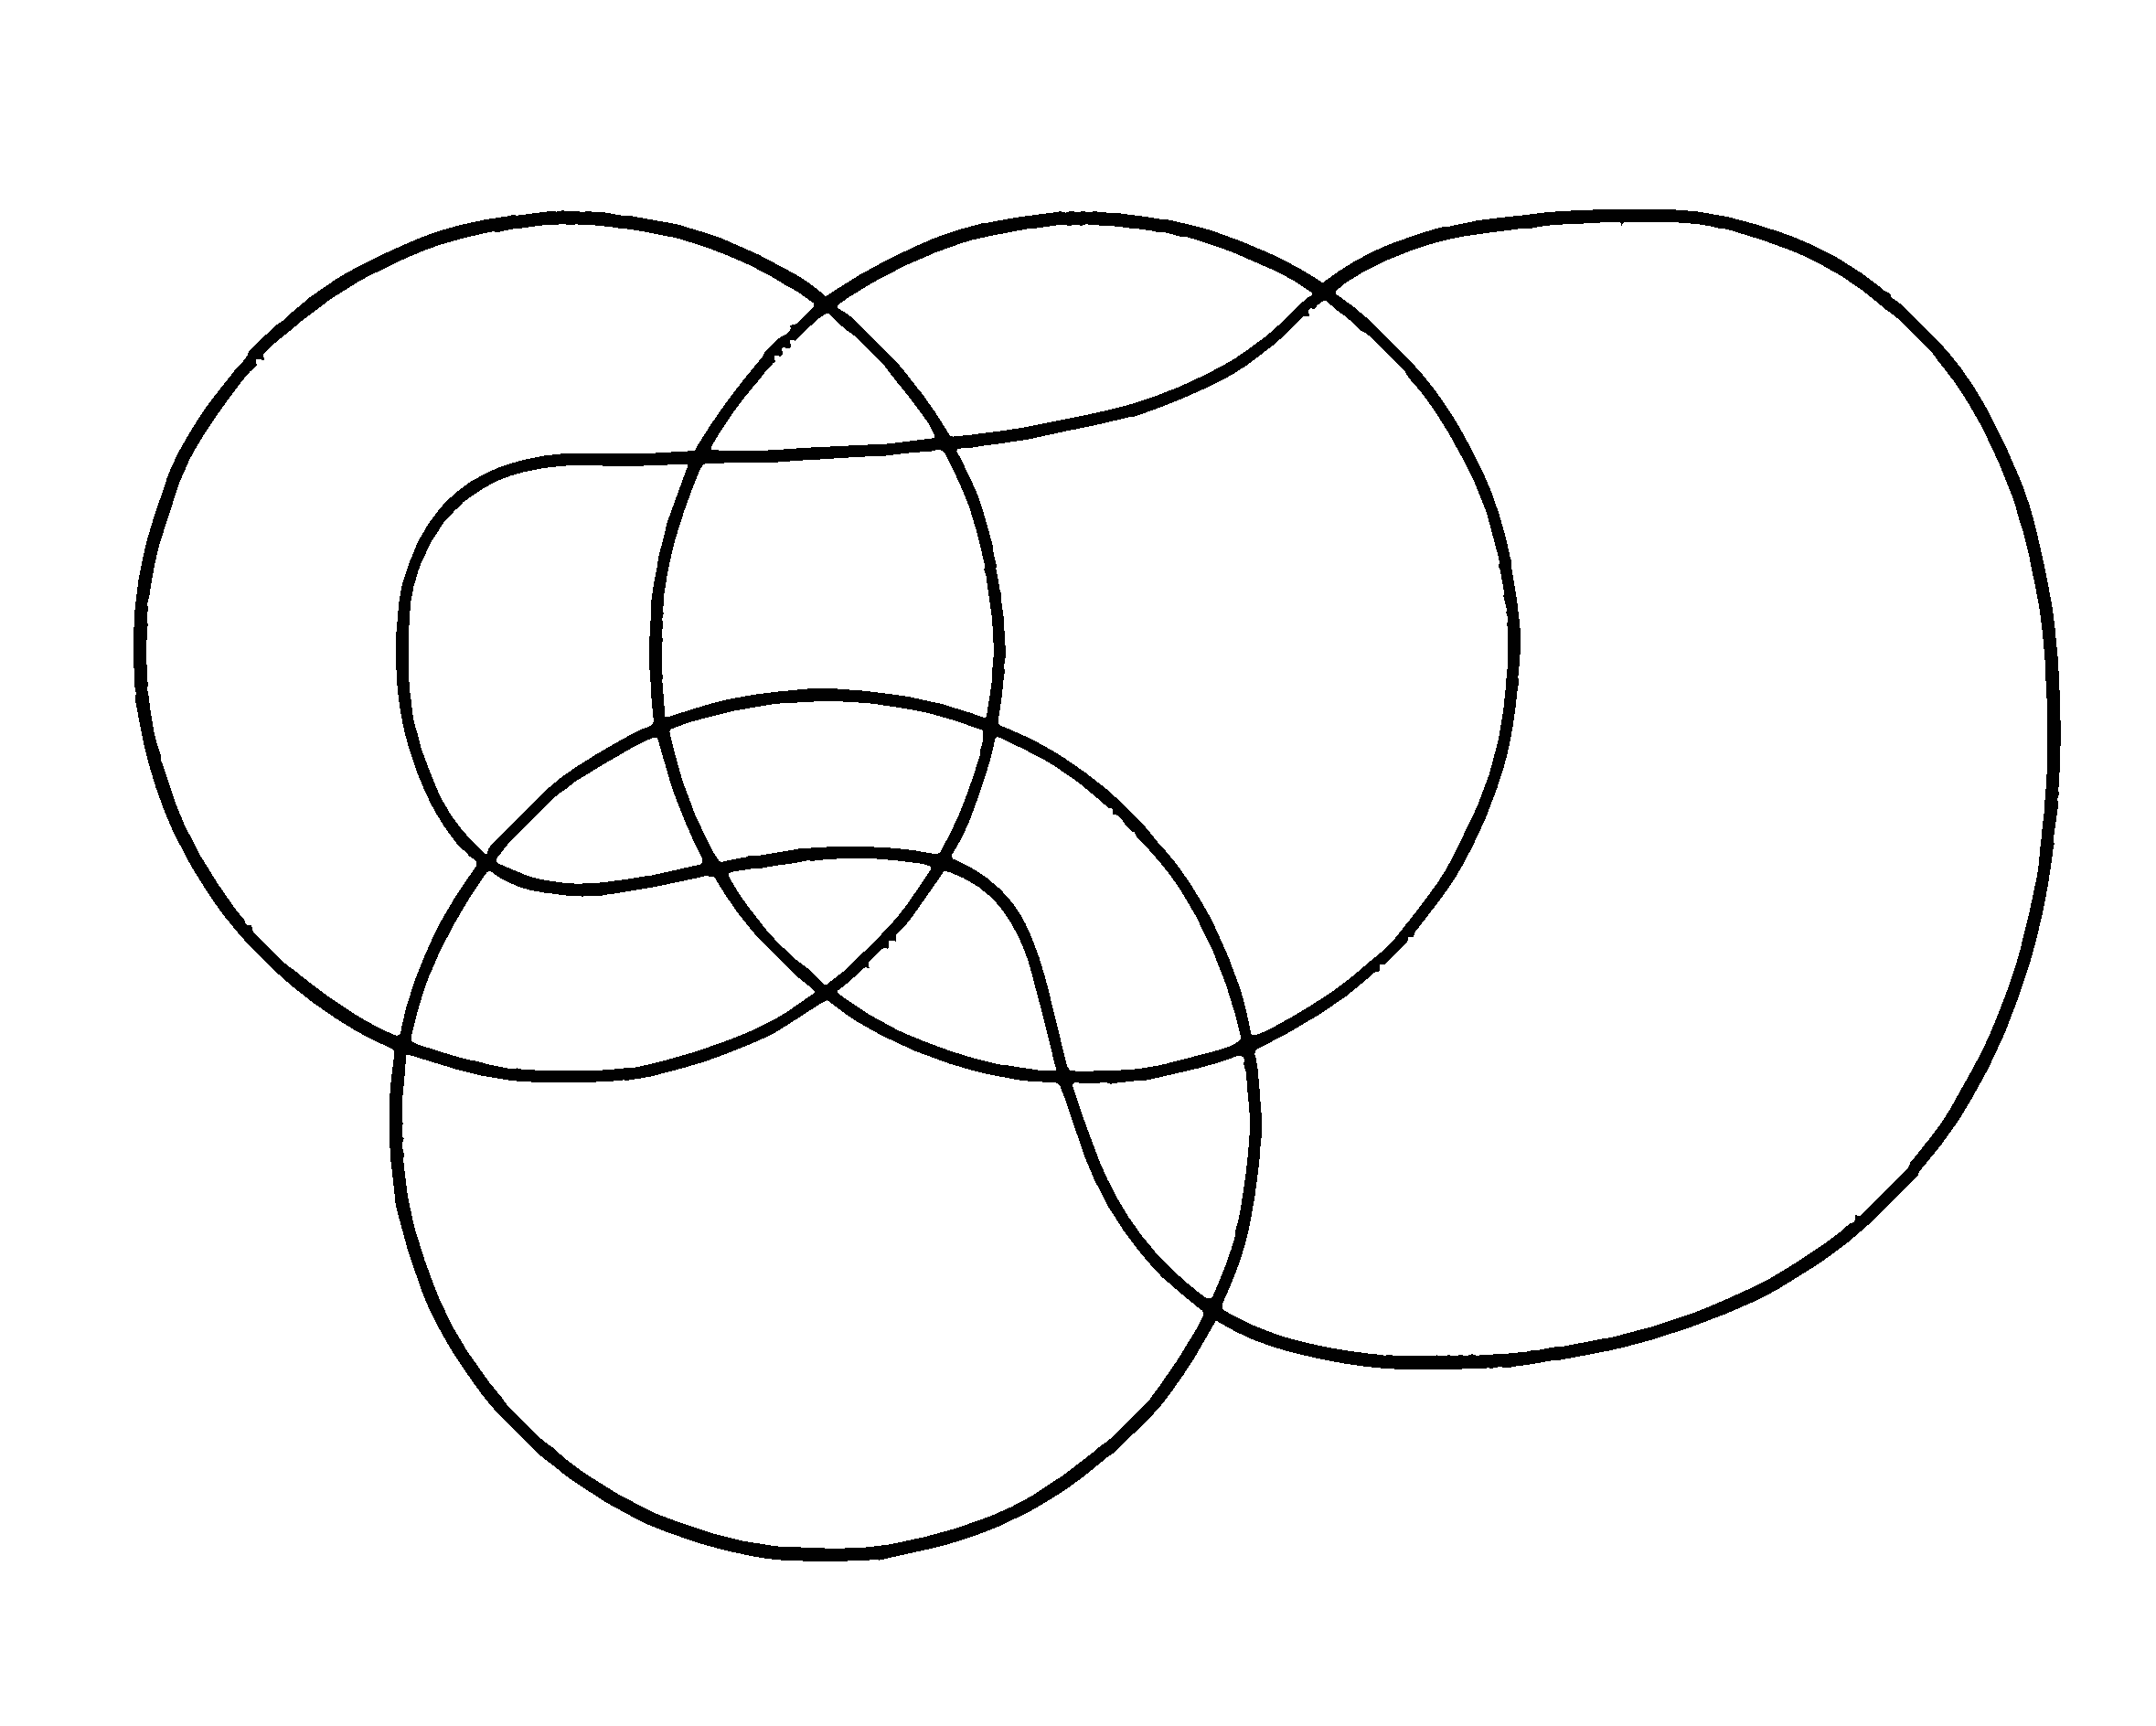
\includegraphics[width=10cm]{Images/MD.pdf}};
        \draw[ultra thick] (-6,-4) node[above right] {$(t = 4)$} rectangle (6,4);
        %\draw (-6,-4) grid (6,4);
        %\filldraw (0,0) circle (2.5pt);
        \node at (-5,2.5) {$1$};
        \node at (-3,2.5) {$2$};
        \node at (0,2.5) {$3$};
        \node at (3,-1) {$4$};
        \node at (-1.5,-2) {$5$};
        \node at (-1.2,2.2) {$6$};
        \node at (-2,-0.5) {$7$};
        \node at (-2.5,1) {$8$};
        \node at (1,1) {$9$};
        \node at (-0.5,-0.5) {$10$};
        \node at (0.45,-1.4) {$11$};
        \node at (-1.2,1.3) {$12$};
        \node at (-2.1,0.25) {$13$};
        \node at (0.1,-0.1) {$14$};
        \node at (-1.2,-0.2) {$15$};
        \node at (-1.2,0.4) {$16$};
        \node[below] at (-1.1,-3.3) {$c_1$};
        \node[above] at (-2.5,3) {$c_2$};
        \node[above] at (0,3) {$c_3$};
        \node[above] at (2.5,3) {$c_4$};
    \end{tikzpicture}
    \caption{~}\label{UAJSBSNZSKKS}
    \end{figure}
\end{itemize}

\begin{BOX}
    Si tomamos un elemento de la región 3, encontramos que se cuenta una vez en $E_1$ y una vez en $S_1$ [en $N\left(c_3\right)$]. Si tomamos un elemento de la región 6, vemos que no se cuenta en $E_1$; se cuenta dos veces en $S_1$ [en $N\left(c_2\right)$ y en $N\left(c_3\right)$] pero se elimina dos veces en $2 S_2$ [ya que se cuenta una vez en $S_2$ en $N\left(c_2 c_3\right)$], por lo que al final no cuenta. El lector debería examinar ahora un elemento de la región 12 y uno de la región 16 y mostrar que cada uno contribuye en 0 a ambos lados de la fórmula para $E_1$.
\end{BOX}

\begin{itemize}[resume]
    \item $E_2$ [regiones 6-11]: De la figura \ref{UAJSBSNZSKKS}, $\displaystyle E_2=S_2-3 S_3+6 S_4=S_2- \binom{3}{1}S_3 + \binom{4}{2} S_4$. Para más detalles sobre esta formula, examinemos los resultados que aparecen en la tabla \ref{JAJABBVVAHXXFTUQOP}, donde junto a cada sumando de $S_2, S_3$ y $S_4$ enumeramos las regiones cuyos elementos se cuentan para determinar ese sumando en particular. Para calcular $S_2-3 S_3+6 S_4$, encontramos los elementos de las regiones 6 a 11, que son precisamente los que se cuentan para $E_2$.
    \begin{center}
        \begin{NiceTabular}[hvlines-except-borders,rules={color=white,width=1pt}]{lll}
        \CodeBefore
        \rowcolor{jblueleft!80}{1}
        \rowcolors{2}{DodgerBlue3!40}{jblueinner}
        \Body
        \RowStyle[color=white]{}
            $S_2$ & $S_3$ & $S_4$ \\
            $N(c_1 c_2)$: 7, 13, 15, 16 & $N(c_1c_2c_3)$: 15, 16 & $N(c_1c_2c_3c_4)$: 16 \\
            $N(c_1 c_3)$: 10, 14, 15, 16 & $N(c_1c_2c_4)$: 13, 16 & \\
            $N(c_1 c_4)$: 11, 13, 14, 16 & $N(c_1c_2c_3)$: 14, 16 & \\
            $N(c_2 c_3)$: 6, 12, 15, 16 & $N(c_2c_3c_4)$: 12, 16 & \\
            $N(c_2 c_4)$: 8, 12, 13, 16 & & \\
            $N(c_3 c_4)$: 9, 12, 14, 16 & & \\
        \end{NiceTabular}
        \captionof{table}{~}\label{JAJABBVVAHXXFTUQOP}
    \end{center}
    \item $E_3$: Por último, los elementos de $E_3$ se encuentra en las regiones 12 a 15 y $\displaystyle E_3 = S_3 - 4S_4 = S_3 - \binom{4}{1}S_4$; los elementos para $E_4$ son los de la región 16 y $E_4 = S_4$.
\end{itemize}